\documentclass[a4paper]{article}
\usepackage[utf8]{inputenc}

\usepackage{amsmath,amssymb}
\usepackage{graphicx}
\usepackage[bf]{subfigure}
\usepackage[bf]{caption}
% Section titles in sans-serif:
\usepackage{sectsty}
\usepackage{abstract}
\allsectionsfont{\sffamily}

%\renewcommand{\abstractname}{\textsf{Abstract} xxxx}
\renewcommand{\abstractnamefont}{\bfseries\textsf}

\usepackage[usenames,dvipsnames]{color}
\definecolor{seagreen}{RGB}{46,139,87}
\definecolor{codebg}{RGB}{255,255,150}
\usepackage{listings}
\usepackage[colorlinks]{hyperref}
\usepackage{url}	

\hypersetup{%
  citecolor=blue,
  linkcolor=blue,
  urlcolor=blue,
}%



\lstset{
  extendedchars=\true,
  inputencoding=utf8,
  language=Matlab,
  %showstringspaces=false,
  formfeed=\newpage,
  tabsize=4,
  %commentstyle=\itshape,
  basicstyle=\ttfamily\scriptsize,
  %basicstyle={\small\fontfamily{fvm}\fontseries{m}\selectfont},
  commentstyle=\color{Apricot}\bfseries,
  %commentstyle=\color{red}\itshape,
  stringstyle=\color{red},
  identifierstyle=\color{PineGreen},
  showstringspaces=false,
  keywordstyle=\color{blue}\bfseries,
  moredelim=[il][\large\textbf]{\#\# },
  morekeywords={models,range},
  numbers=left,
  numbersep=2pt,
  numberstyle=\tiny,%\color{blue}\bfseries,
  backgroundcolor=\color{codebg},
  literate=%
  {ã}{{\~a}}1
  {â}{{\^a}}1
  {õ}{{\~o}}1
  {á}{{\'a}}1
  {ú}{{\'u}}1
  {í}{{\'i}}1
  {é}{{\'e}}1
  {Ç}{{\c{C}}}1
  {Õ}{{\~O}}1
  {Ê}{{\^E}}1
  {ó}{{\'o}}1
  {à}{{\`a}}1
  {Â}{{\^A}}1
  {ô}{{\^o}}1
  {ê}{{\^e}}1
  {ç}{{\c{c}}}1
}

\newcommand{\code}[2]{
 \vspace{1em}
 \subsubsection*{#1}
 \lstinputlisting{#2}
}

%%%%%%%%%%%%%%%%%%%%%%%%%%%%%%%%%%%%%%%%
% You have two versions of the macro
% \draftnote{My note}. The first version puts notes (e.g. My note in the example)
% into the margin of your document. The second formats the note as nothing. You
% 'comment out' the version of the macro you don't want (using a % at the
% beginning of the line).
\newcommand{\draftnote}[1]{\marginpar{\tiny\raggedright\textsf{\hspace{0pt}#1}}}
%\newcommand{\draftnote}[1]{}

% This one is just for the comments for in-line text.
\newcommand{\indraftnote}[1]{\textcolor[HTML]{114406}{\texttt{\footnotesize[#1]}}}
%\newcommand{\indraftnote}[1]{}
\newcommand{\todo}[1]{\indraftnote{todo: #1}}
\newcommand{\ie}{{\it i.e.}}
\newcommand{\etc}{{\it etc}}
\newcommand{\eg}{{\it e.g.}}
\newcommand{\wrt}{{\it w.r.t. }}
\newcommand{\etal}{{\it et.\ al.\ }}
\newcommand{\etalf}{{\it et.\ al.}}


\begin{document}

\title{\textsf{Computer Vision Lab \#2\\ Hough Transform}
\marginpar{\vspace{-1.2cm}
\includegraphics[height=1.4cm] {figs/logo_uerj_cor_small.png}}} 

\author{Prof.\ Ricardo Fabbri, Ph.D.\footnote{Based on Image Understanding
2011 lab material from Ben Kimia, Brown University}\\[1em]
Polytechnic Institute at the Rio de Janeiro State University\\
\url{http://wiki.nosdigitais.teia.org.br/CV}
}
 

\date{\today}
\maketitle
\begin{abstract}
\noindent\begin{itemize}
\item Detect lines and circles in an image using the Hough transform
\item Implement your own version and compare to SIP and OpenCV
\end{itemize}
\end{abstract}
\vspace{2em}



The images you will need for the lab can be downloaded from the course
website. All extra work will be considered for bonus grade points.

\section{Implement the Hough Transform for Multiple Line Detection}

In this problem, you will implement the Hough Transform to detect lines, see
Figure~\ref{fig:img5}.
\begin{figure}[t]
\centering
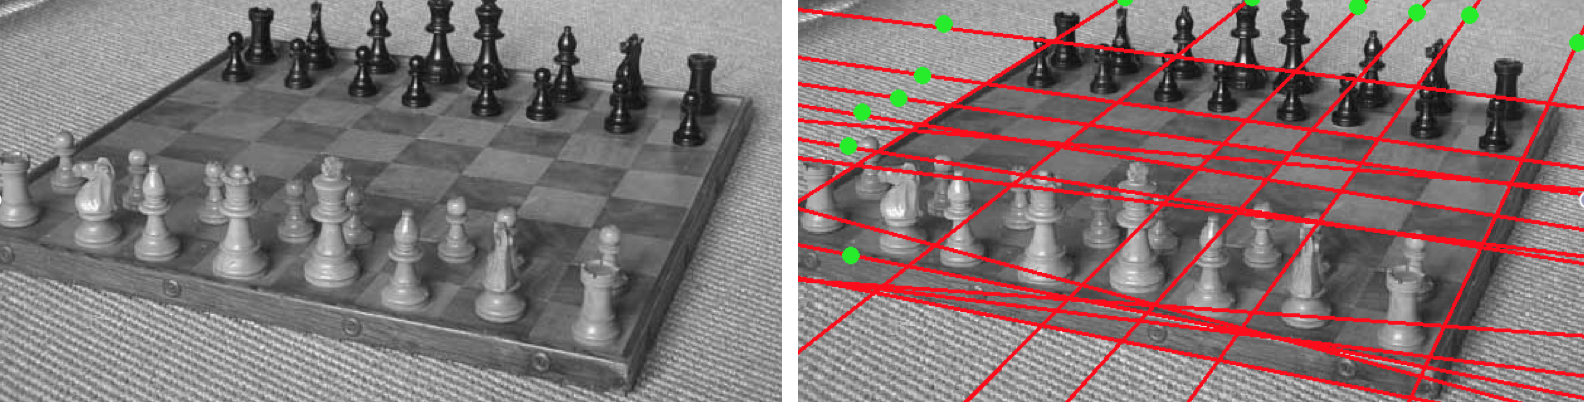
\includegraphics[width=0.8\linewidth]{figs/line-hough.png}%
\caption{% 
(left) Checkerboard image (right) Sample output of line Hough transform
}\label{fig:img5}
\end{figure}
We will use the normal form of a line, Equation~\ref{eq:eq5}, as explained in
class
\begin{equation}\label{eq:eq5}
\rho = x\cos\theta + y\sin\theta
\end{equation}
The pseudocode for the Hough transform algorithm is as follows

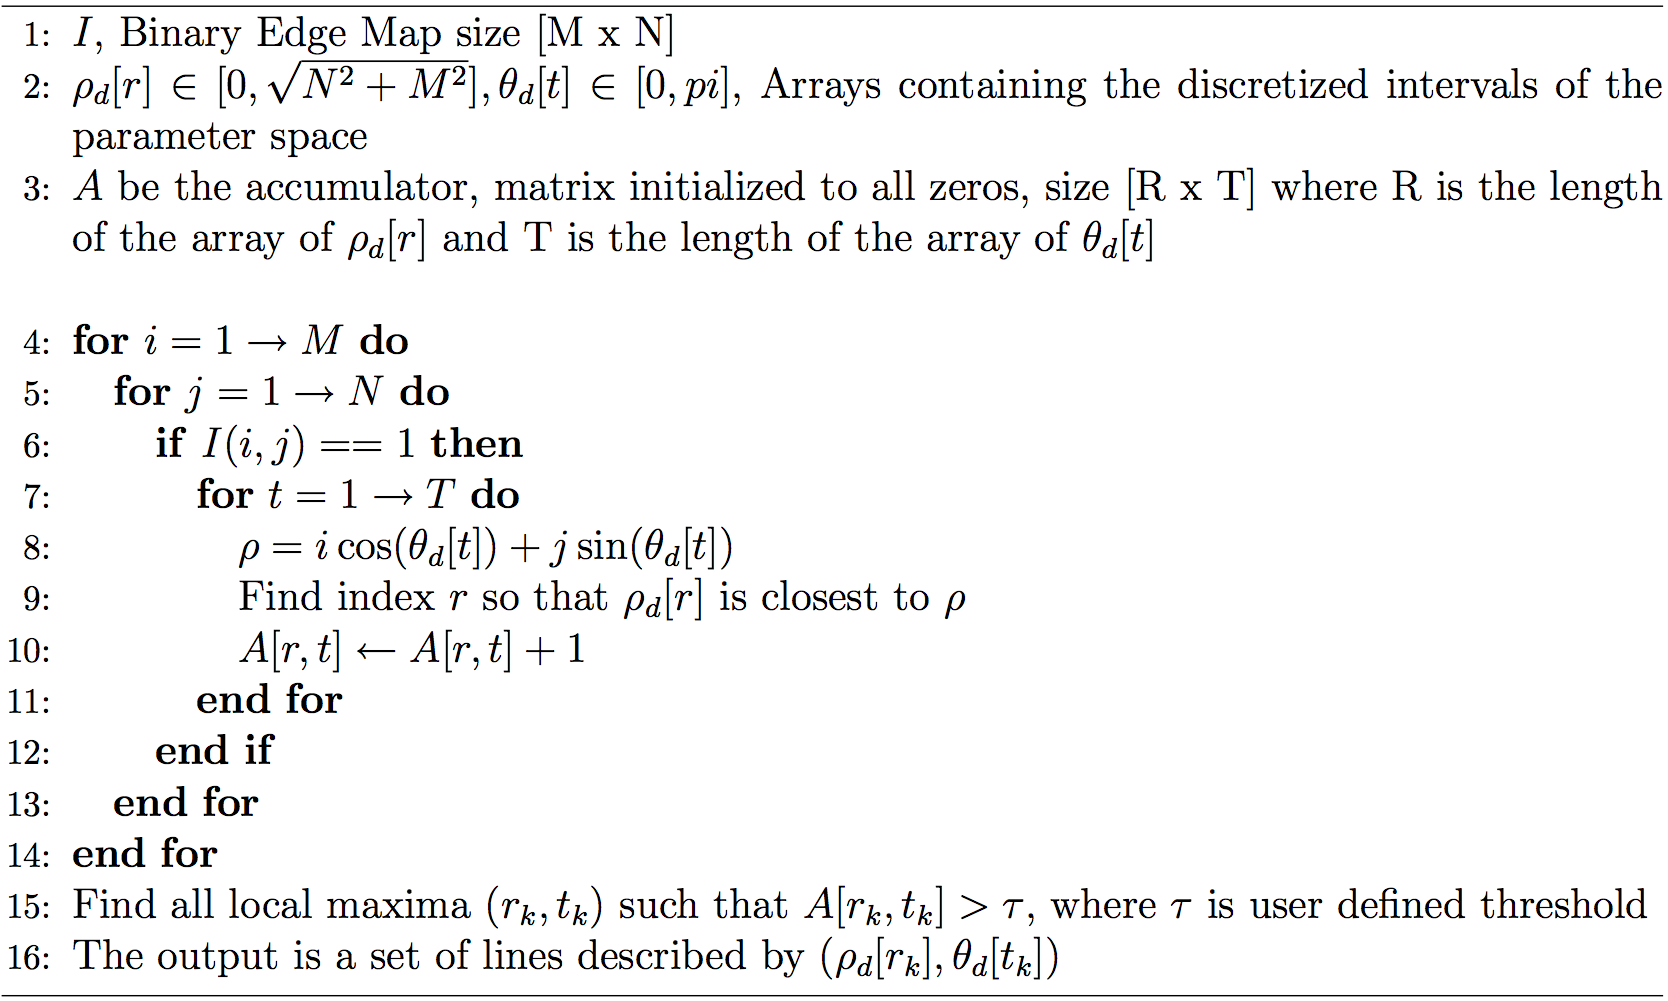
\includegraphics[width=1\linewidth]{figs/alg-hough-lines.png}%

\paragraph{Some comments on lines of the algorithm:}
\begin{itemize}
\item[Line 1:] This is the output of a gradient-based edge
detector. You can use SIP's \texttt{edge} function with the Sobel operator. Does
the algorithm work better if you use \texttt{thin} on top of the edge image?
Show the edge images for all results.
\item[Line 2:] When you define these arrays you are discretizing the parameter
space of $\rho$ and $\theta$ using steps of $\Delta \rho$ and $\Delta
\theta$. Choose appropriate step sizes that yield acceptable and manageable
resolution of the parameter space.
\item[Line 9:] The value computed for $\rho$ will not exactly be in your
parameter space, so you have to choose either to round, ceil, or floor the value.
\item[Line 15:] When defining your threshold, think about how many edge points would
have to vote for a line.
\end{itemize}
Requirement for your report:
\begin{enumerate}
\item Display your accumulator space A as an image. This is also called a
sinogram.
\item Plot all lines found on top of 3 different images of your choice
(buildings, mechanical pieces), such as those in
Figure~\ref{fig:line:hough:imgs}. You can use SIP's \texttt{imshow} followed by a
plot command, as long as you set the plot to be persistent.
\begin{figure}
\centering
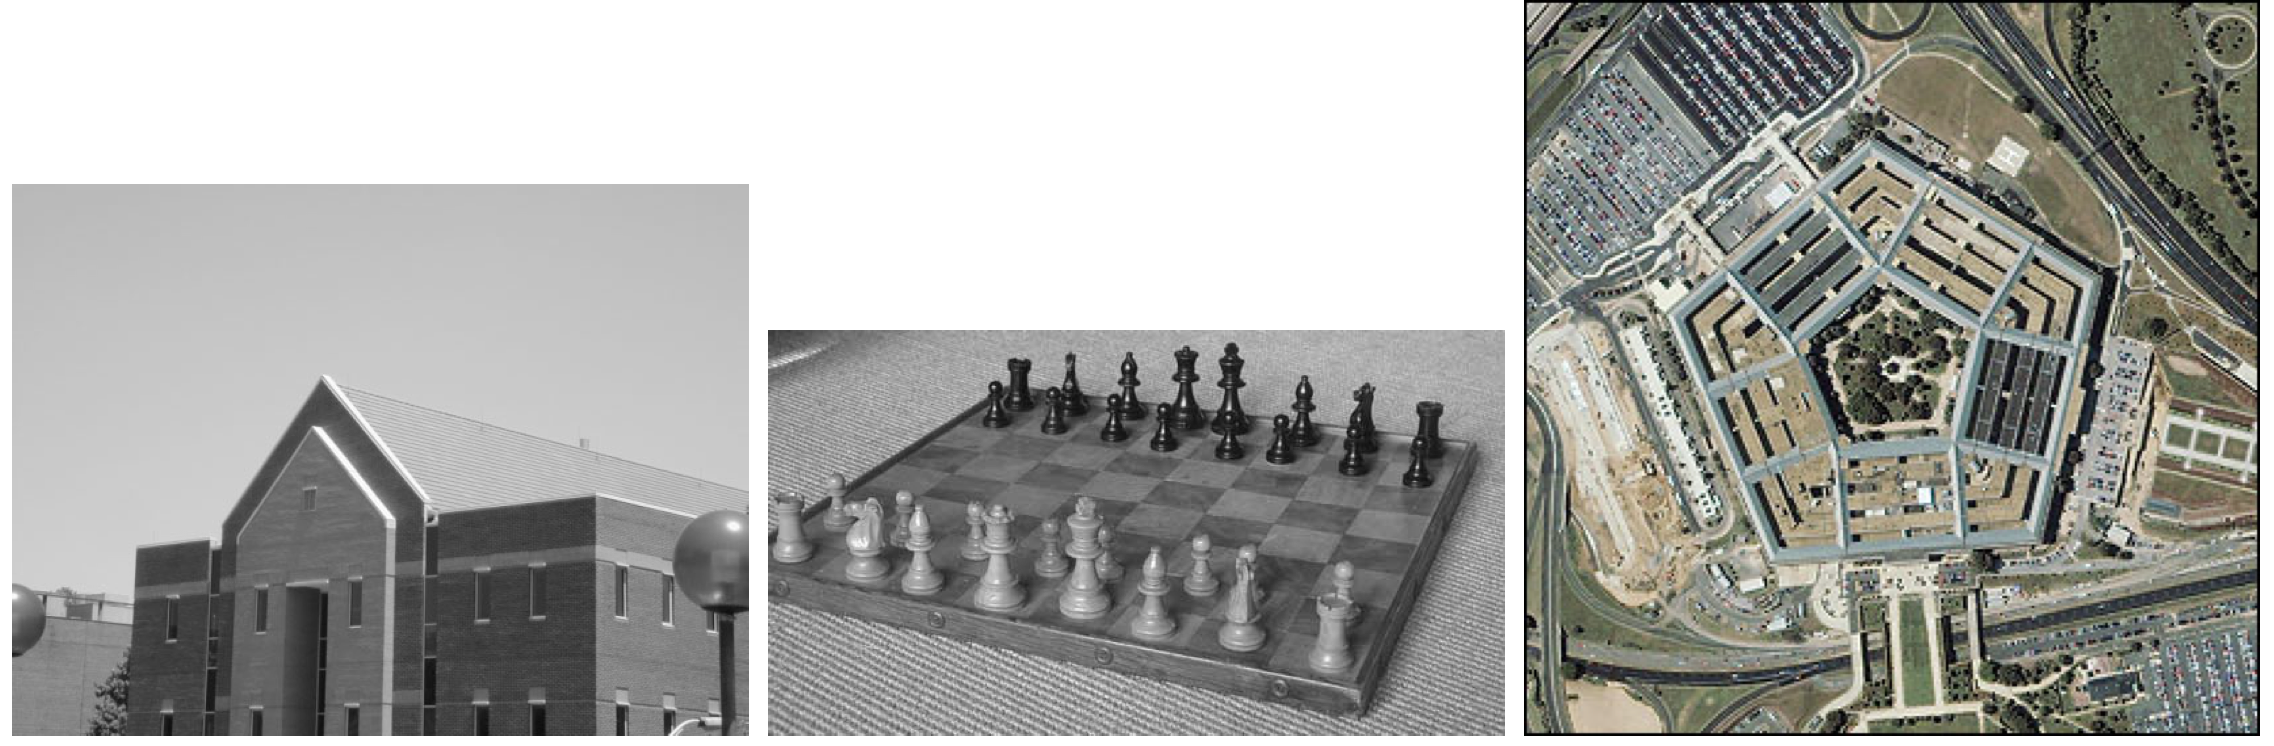
\includegraphics[width=\linewidth]{figs/images-for-line-hough.png}%
\caption{% 
You should run your line detection algorithm on these images or very similar ones.
}\label{fig:line:hough:imgs}
\end{figure}
\item What does an edge point $(x,y)$ in the image correspond to in the $(\rho,
theta)$ parameter space?
\item Comment on the effect of discretization of the parameter space, and the
threshold you used
\item If you were to implement this multiple line detection with RANSAC, what type of shortcomings can
you predict? How would you use RANSAC to detect multiple lines?
\item Compare your implementation to SIP's \texttt{hough} and \texttt{ihough}
functions. What are some flaws of SIP's code that you can see?
\end{enumerate}

\section{Implement Hough Transform for Multiple Circle Detection} The Hough transform is a very
general approach that we can use to detect any shape that has (short) a
parametric form! We sill use the same aforementioned approach but now to detect
circles, see Figure~\ref{fig:hough:circles}.  A circle with radius $r$ and
center $(a,b)$ can be described with parametric equations,
Eq.~\ref{eq:circle:parametric}.
\begin{equation}\label{eq:circle:parametric}
\left\{\begin{aligned}
x &= a + r\cos\theta\\
y &= b + r\cos\theta
\end{aligned}\right.
\end{equation}
\begin{figure}[h]
\centering
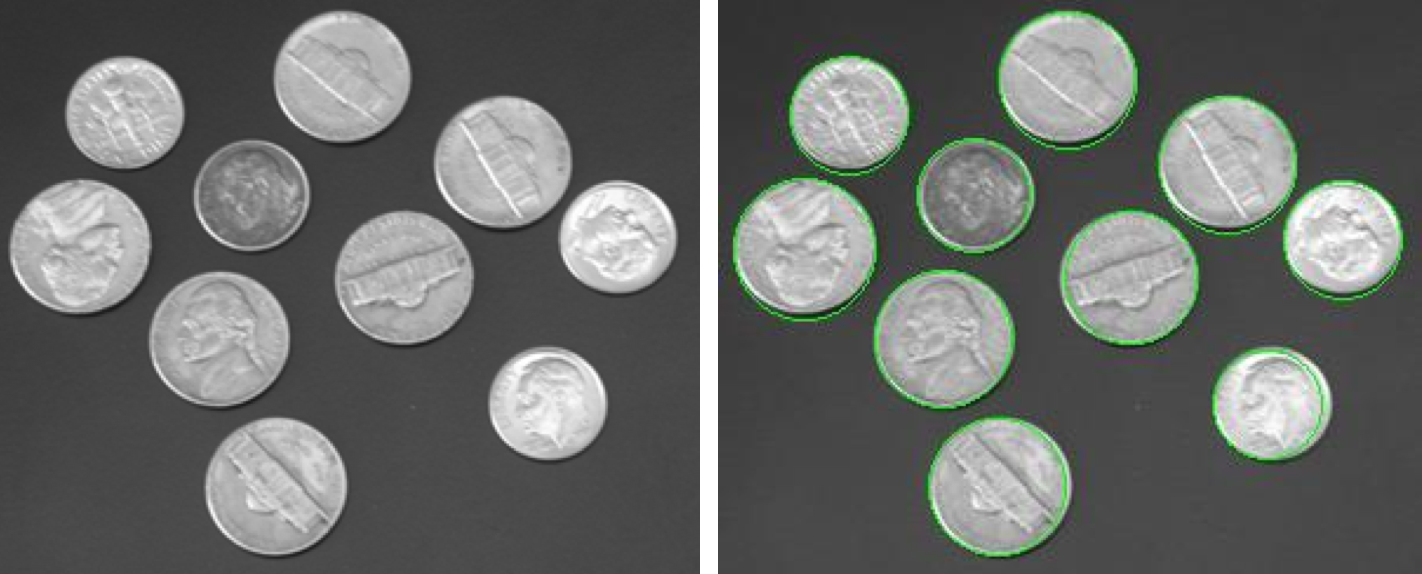
\includegraphics[width=0.8\linewidth]{figs/circular-hough.png}%
\caption{% 
(left) Input of coins, (right) Sample output of circle Hough transform.
}\label{fig:hough:circles}
\end{figure}
If an image contains many points $(x,y)$, some of which fall on the perimeters of
circles, then the job of the search program is to find parameter triplets
$(a,b,r)$ to describe each circle. We will use the same approach as in Algorithm
2 for lines.
Some comments on lines of the Hough algorithm:
\begin{itemize}
\item[Line 2:] Here you will have three arrays that define the discretization
of $a_d, b_d, r_d$.
\item[Line 3:] Your accumulator will be a 3D matrix of all zeros, again, the
size of it will be
$\text{length}(a_d)\times\text{length}(b_d)\times\text{length}(r_d)$, the 3D
case will be more expensive in terms of both time and memory, so be
judicious in your discretization of the parameter space
\item[Line 7:] To evaluate Equation~\ref{eq:circle:parametric} you will have two
loops instead of one, one loop will be over $r_d$ and the other will be over a
discretization of $\theta$, where $\theta$ ranges from 0 to $2\pi$.
\item[Line 9:] After evaluating Equation~\ref{eq:circle:parametric} you will
have two parameters $a,b$ and you will again have to find the closest bin in the
3D accumulator $A[i,j,k]$, keeping in mind you are looping over $r_d$ so you
already know the index of one parameter.
\item[Line 15:] When defining your threshold, think about how many edges would
have to vote for a circle. Also keep in mind you have to look around 3
dimensions when finding the local maxima
\end{itemize}
Requirement for your report:
\begin{enumerate}
\item Plot all found circles on top of the input images of
Figure~\ref{fig:images:circle:hough}. There are many options to plot a circle on
top of an image, you can use \texttt{plot} on top of \texttt{imshow} or even use
SIP's \texttt{mogrify} to draw a circle directly in the image (as in the mogrify
demo).
\item What does an edge point $(x,y)$ in the image correspond to in the
$(a,b,r)$ parameter space?
\item Comment on the effect of discretization of the parameter space, and the
threshold you used
\end{enumerate}
\begin{figure}
\centering
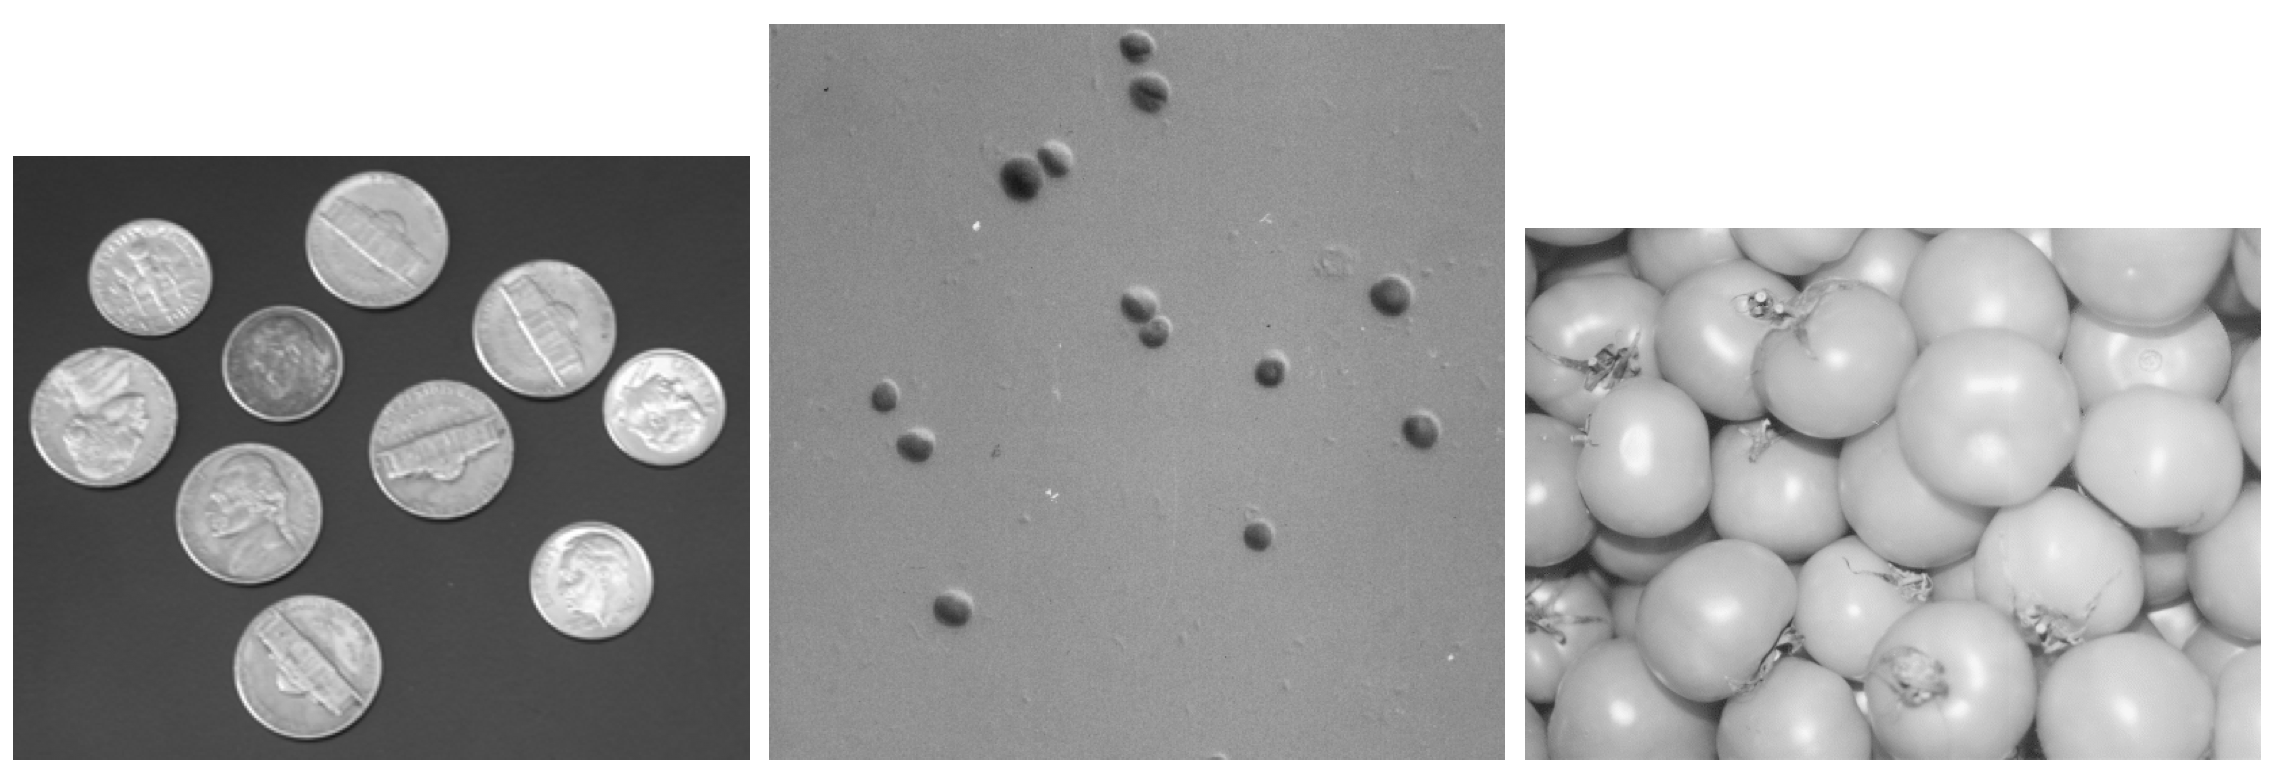
\includegraphics[width=\linewidth]{figs/images-for-circle-hough.png}%
\caption{% 
You should run your circle detection algorithm on these images or very similar ones.
}\label{fig:images:circle:hough}
\end{figure}

\section{Comparison with OpenCV}
\begin{enumerate}
\item Install OpenCV from Git following instructions at \url{http://wiki.nosdigitais.teia.org.br/OpenCV}
\item Learn how to run OpenCV hough transform functions from the commandline,
for both circles and lines
\item Compare the results and performance with your implementation. Report
running times and mainly on the quality of the output.
\item Bonus: open the source code for the hough transform in OpenCV. What can
you identify? Describe two optimization tricks being used.
\end{enumerate}

\paragraph{Bonus Challenge -- Accelerated Hough Transform -- 3 extra points} One way of reducing the
computation required to perform the Hough transform is to make use of gradient
information (magnitude and/or direction) which is often available as output from
an edge detector.  Explain in detail how you would use the gradient to
accelerate the Hough transform, and provide an implementation.



\bibliographystyle{IEEEtran}
\bibliography{personal}

\end{document}
